%%%%%%%%%%%%%%%%%%%%%%%%%%%%%%%%%%%%%%%%%
% Thin Sectioned Essay
% LaTeX Template
% Version 1.0 (3/8/13)
%
% This template has been downloaded from:
% http://www.LaTeXTemplates.com
%
% Original Author:
% Nicolas Diaz (nsdiaz@uc.cl) with extensive modifications by:
% Vel (vel@latextemplates.com)
%
% License:
% CC BY-NC-SA 3.0 (http://creativecommons.org/licenses/by-nc-sa/3.0/)
%
%%%%%%%%%%%%%%%%%%%%%%%%%%%%%%%%%%%%%%%%%

%----------------------------------------------------------------------------------------
%	PACKAGES AND OTHER DOCUMENT CONFIGURATIONS
%----------------------------------------------------------------------------------------

\documentclass[a4paper, 11pt]{article} % Font size (can be 10pt, 11pt or 12pt) and paper size (remove a4paper for US letter paper)
\usepackage{color}
\usepackage[protrusion=true,expansion=true]{microtype} % Better typography
\usepackage{graphicx} % Required for including pictures
\usepackage{wrapfig} % Allows in-line images
\usepackage{endnotes}
\usepackage{mathpazo} % Use the Palatino font
\usepackage[T1]{fontenc} % Required for accented characters
\linespread{1.05} % Change line spacing here, Palatino benefits from a slight increase by default
\usepackage{fancyhdr}
\usepackage[margin=1.25in]{geometry}
\pagestyle{fancy}
\fancyhf{}
\rhead{Machine Learning Problem Set 2, 14.02.2019}
\lhead{Felix Adam}
\rfoot{Page \thepage}
\usepackage{amsmath}
\usepackage{amssymb}
\usepackage{version}
\usepackage{setspace}
\usepackage{enumerate}
\usepackage{multicol}
\usepackage{amsfonts}
\usepackage{amssymb}
\usepackage{graphicx}
\usepackage{rotating}
\usepackage{lscape}
\usepackage{pdflscape}
\usepackage{array,tabularx,float,dcolumn,lscape}
\usepackage{booktabs}
\usepackage{xr}
\usepackage{dcolumn}
\usepackage{hyperref} 
\usepackage{amsmath}
\usepackage{algorithm}
\usepackage[noend]{algpseudocode}
\graphicspath{ {../01_Figures/} }

\makeatletter
\def\BState{\State\hskip-\ALG@thistlm}
\makeatother

\newlength\tindent
\setlength{\tindent}{\parindent}
\setlength{\parindent}{0pt}
\renewcommand{\indent}{\hspace*{\tindent}}
\renewcommand{\familydefault}{\sfdefault}

\makeatletter
\renewcommand\@biblabel[1]{\textbf{#1.}} % Change the square brackets for each bibliography item from '[1]' to '1.'
\renewcommand{\@listI}{\itemsep=0pt} % Reduce the space between items in the itemize and enumerate environments and the bibliography

\renewcommand{\maketitle}{ % Customize the title - do not edit title and author name here, see the TITLE block below
\begin{flushright} % Right align
{\LARGE\@title} % Increase the font size of the title

\vspace{50pt} % Some vertical space between the title and author name

{\large\@author} % Author name
\\\@date % Date

\vspace{40pt} % Some vertical space between the author block and abstract
\end{flushright}
}

\begin{document}

\section*{Problem 5} 

\subsubsection*{Bayes Classifier}

In order to derive the Bayes classifier, we need to compute the posterior probability $\eta ( x ) = P ( y = 1 | X = x )$. Using Bayes rule, we can define 

$$\eta(x) = \frac{P(X \leq x | Y = 1) P(Y = 1)}{P(X\leq x)}$$

where we can use the law of total probability to find $P(X=x)$. Given the problem, we know that $\mathbf { P } ( Y = 0 ) = \mathbf { P } ( Y = 1 ) = 1 / 2$ and the conditional cumulative distributions:

$$\mathbf { P } \{ X \leq x | Y = 0 \} = \left\{ \begin{array} { l l } { 0 } & { \text { if } x \leq 0 } \\ { x ^ { 2 } / 4 } & { \text { if } 0 < x \leq 2 } \\ { 1 } & { \text { if } x > 2 } \end{array} \right.$$

$$\mathbf { P } \{ X \leq x | Y = 1 \} = \left\{ \begin{array} { l l } { 0 } & { \text { if } x \leq 1 } \\ { ( x - 1 ) / 2 } & { \text { if } 1 < x \leq 3 } \\ { 1 } & { \text { if } x > 3 } \end{array} \right.$$

Therefore we can derive $P(X=x)$ for the given intervals. The probability density functions following from the CDFs are the following:

$$f_{Y=0} = \left\{ \begin{array} { l l } { 0 } & { \text { if } x \leq 0 } \\ { x  / 2 } & { \text { if } 0 < x \leq 2 } \\ { 0 } & { \text { if } x > 2 } \end{array} \right.$$

$$f_{Y=1} = \left\{ \begin{array} { l l } { 0 } & { \text { if } x \leq 1 } \\ { 1/2} & { \text { if } 1 < x \leq 3 } \\ { 0 } & { \text { if } x > 3 } \end{array} \right.$$

The unconditional distribution of $X$ has the following form:

$$f_x = \left\{ \begin{array}{ ll} {0} & {\text {if } x \leq 0} \\ 
{\frac{x}{4}} & {\text{if } 0 < x \leq 1  } \\
{\frac{x+1}{4}} & {\text {if } 1 < x \leq 2} \\
{\frac{1}{4}} & { \text {if } 2 < x \leq 3} \\
{0} & {\text {if } x > 3 } \end{array} \right. $$

We can now use this to calculate $\eta(x)$.

$$\eta(x) = \left\{ \begin{array}{ ll} {0} & {\text {if } x < 1} \\ 
{\frac{1}{x+1}} & {\text{if } 1 < x \leq 2  } \\
{1} & {\text{if } 2 < x \leq 3  } \\
{0} & {\text{if }  x > 3  }
\end{array} \right. $$

In the interval $1 x \leq 2$, $\eta(x)$ is never bigger than $1/2$. Following, the Bayes classifier is :

$$g^*(x) = \left\{ \begin{array}{ ll} {0} & {\text {if } 0 < x \leq 2} \\
{0} & {\text{if } 1 < x \leq 2 } \\
{1} & {\text{if } 2 < x \leq 3 } \\
{0} & {\text{else } }
\end{array} \right. $$

The Risk is the expected loss over the whole interval.In the intervals of $0 < x \leq 2$ and $2 < x \leq 3 $ the probability of error is zero. In the interval $1 < x \leq 2$ we define the expected loss as

\begin{align*}
E\left[l(g^*(x),y) \right]  &= E\left[ P\left(g^*=0 , Y=1 | X\right) +  P\left(g^*=1 , Y=0 | X\right) \right ]\\
&=E \left[ \mathbb{1}_{(g^*=0)} P\left(Y=1 | X\right) +\mathbb{1}_{(g^*=1)} P\left(Y=0 | X\right) \right] \\
&= E \left[ \mathbb{1}_{(g^*=0)} \eta(x) +\mathbb{1}_{(g^*=1)} (1-\eta(x)) \right]
\end{align*}

(Assuming symmetric, 0-1 loss). Consequently, the risk is 

$$R ^ { * } = \left\{ \begin{array} { l l } { 0 } & { \text { if } 0 < x \leq 1 } \\ {E [ \min ( \eta ( x ) , 1 - \eta ( x ) ) ] } & { \text { if } 1 < x \leq 2 } \\ { 0 } & { \text { if } 2 < x \leq 3 } \end{array} \right.$$

We can calculate the expected loss in the interval $1 < x \leq 2$:

$$E_{(1 < x \leq 2)}[\eta(x)] = \int _ { 1 } ^ { 2 } \eta ( x ) P ( X = x ) = \int _ { 1 } ^ { 2 } \frac { 1 } { 1 + x } \frac { x + 1 } { 4 } = \frac { 1 } { 4 }$$

since we know that $\eta(X) < 1-\eta(x)$ for all $1<x<2$ 

Finally we can write the risk as:

$$R ^ { * } = \left\{ \begin{array} { l l } { 0 } & { \text { if } 0 < \mathrm { x } \leq 1 } \\ { 1 / 4 } & { \text { if } 1 < \mathrm { x } \leq 2 } \\{ 0 } & { \text { if } 2 < \mathrm { x } \leq 3 } \end{array} \right.$$

\subsubsection*{Risk of 1-NN Classifier}

The risk of the 1-NN Classifier is derived using the formula we found in class: 

$$R ^ { 1 - N N } = E [ 2 \eta ( x ) ( 1 - \eta ( x ) ) ]$$ 

In this case, again the only overlap between the two densities is in the interval $1 < \mathrm { x } \leq 2$. In the other cases, the asymptotic risk that the nearest neighbor is not of the same class is zero. So we only need to calculate the risk for said interval. Taking expectations we get:

\begin{align*}
E \left[ 2 \frac { 1 } { 1 + x } \frac { x } { 1 + x } \right] = \int _ { 1 } ^ { 2 } \frac { 2 x } { ( x + 1 ) ^ { 2 } } \frac { 1 + x } { 4 } &= \int _ { 1 } ^ { 2 } \frac { x } { 2 ( x + 1 ) } \\
&=  \frac { 1 } { 2 } \left[ x - \ln ( x + 1 ) \right] _ { 1 } ^ { 2 }\\
&= \frac{1}{2} \left(1 + \ln \left(\frac{2}{3} \right) \right) \approx 0.3
\end{align*}


\section*{Problem 6} 

The optimal ranking rule is the following:
$$
g^*(x) = \left\{ \begin{array}{ ll} {1} & {\text {if } \eta(x) > \eta(x')} \\
{0} & {\text{if } \eta(x) < \eta(x') } \\
\end{array} \right. $$

If the posterior probability of $x$ being one is bigger than the posterior of $x'$ being one, rank $x$ higher than $x'$ and vice versa.

The risk of this rule is:

\begin{align*}
P(g^* \neq Z) &= P(g^*(x,x') = 1, y = 0, y'=1 | x, x') + P(g^*(x,x') = 0, y = 1, y'=0 | x, x') \\
&= \mathbb{1}_{(g(x,x') = 1)} P(y = 0, y'=1 | x, x') + \mathbb{1}_{(g(x,x') = 0)} P(y = 1, y'=0 | x, x') \\
&= \mathbb{1}_{(g(x,x') = 1)} P(y = 0| x)P(y'=1 |x') + \mathbb{1}_{(g(x,x') = 0)} P(y = 1| x)P(y'=0 | x') \\
&= \mathbb{1}_{(g(x,x') = 1)} (1-\eta(x))\eta(x') + \mathbb{1}_{(g(x,x') = 0)} \eta(x) (1-\eta(x'))
\end{align*}

Where $Z$ represents the true ranking (noting that no loss occurs if both classes are equal). Consequently the risk of the rule is:

$$E\left[ l(g^*,x) \right] = E\left[ min((1-\eta(x))\eta(x'),\eta(x) (1-\eta(x')\right]$$


\section*{Question 7}

\subsubsection*{Bayes Classifier}

The question states, that the probability of a given observation $X$ being of class $Y=1$, is a random Bernoulli variable with probability $p$ equal to the first entry of the vector describing the observation. Therefore the Bayes rule predicts that $Y =1$ if the first entry is greater than $1/2$ and $Y=0$ else. 

Formally,

$$g^*(x) = \left\{ \begin{array}{ ll} {1} & {\text {if } \eta(x) = x ^ { ( 1 ) } >  1/2 } \\
{0} & {\text{if } \eta(x) = x ^ { ( 1 ) }   \leq 1/2 } \\
\end{array} \right. $$

where $\eta(x) = \mathbf { P } \{ Y = 1 | X = x \} = x ^ { ( 1 ) }$.

The Bayes risk is again the expected loss:
An error occurs if either we predict $g(x) = 1$ in which case $x^{(1)} > 0.5$ or vice versa $g(x) = 0$ and $x^{(1)} \leq 0.5$. Thus the risk of the Bayes classifier is


$$E\left[l(g^*,y)\right] = \mathbb{1}_{g(x) = 1}E[1- \eta(x)| x>0.5  ] + \mathbb{1}_{g(x) = 0} E[ \eta(x) | x <0.5 ]$$

We know that $x$ is uniformly $[0,1]$ distributed so we get: 

$$E[\eta(x) | x \leq 0.5] = \int _ { 0 } ^ { 1 / 2 } 2 x d x = \left[ x ^ { 2 } \right] _ { 0 } ^ { 1 / 2 } = 1 / 4$$

and

$$E[1 -\eta(x) | x > 0.5] = \int _ { 1/2 } ^ { 1 } 2 (1-x) d x =  2\left[ 1x - x ^ { 2 } \right] _ { 1/2 } ^ { 1 } = 1 / 4$$


Therefore the Bayes risk is $E\left[l(g^*,y)\right] = \frac{1}{4}$.

\subsubsection*{Nearest Neighbor Classifiers}

For the risk of the 1-NN Classifier we can again use the formula from class: $R ^ { 1 - N N } = E [ 2 \eta ( x ) ( 1 - \eta ( x ) ) ]$

Plugging in $\eta(x) =  x ^ { ( 1 ) }$ we get:

\begin{align*}
R ^ { 1 - N N } &= 2 \int _ { 0 } ^ { 1 } x ( 1 - x ) d x \\
&= 2\int _ { 0 } ^ { 1 } x - x ^ { 2 } d x \\
&= 2 \left[ \frac { x ^ { 2 } } { 2 } - \frac { x ^ { 3 } } { 3 } \right] _ { 0 } ^ { 1 } \\
&= 2 \left[ \frac { 1 } { 2 } - \frac { 1 } { 3 } \right]  = \frac{1}{3}
\end{align*}

Similarly, for the risk of the 3-NN Classifier, we use the formula from class $E [ \eta ( x ) ( 1 - \eta ( x ) ) ] + E \left[ 4 \eta ( x ) ^ { 2 } ( 1 - \eta ( x ) ) ^ { 2 } \right]$ and get for the risk

\begin{align*}
R ^ { 3 - N N } &=\int _ { 0 } ^ { 1 } x ( 1 - x ) d x + 4 \int _ { 0 } ^ { 1 } x ^ { 2 } \left( 1 - 2 x + x ^ { 2 } \right) d x \\
&= \frac { 1 } { 6 } + 4 \int _ { 0 } ^ { 1 } x ^ { 2 } - 2 x ^ { 3 } + x ^ { 4 } d x \\
&= \frac { 1 } { 6 } + 4 \left[ \frac { x ^ { 3 } } { 3 } - 2 \frac { x ^ { 4 } } { 4 } + \frac { x ^ { 5 } } { 5 } \right] _ { 0 } ^ { 1 } = \frac{3}{10}
\end{align*}

\newpage
\subsection*{Simulations}

For the simulations we see, that risk converges very quickly towards the asymptotic risk, but only in lower dimensions. In high dimensions, the risk converges slowly even for larger samples.

\begin{figure}[H]
\centering
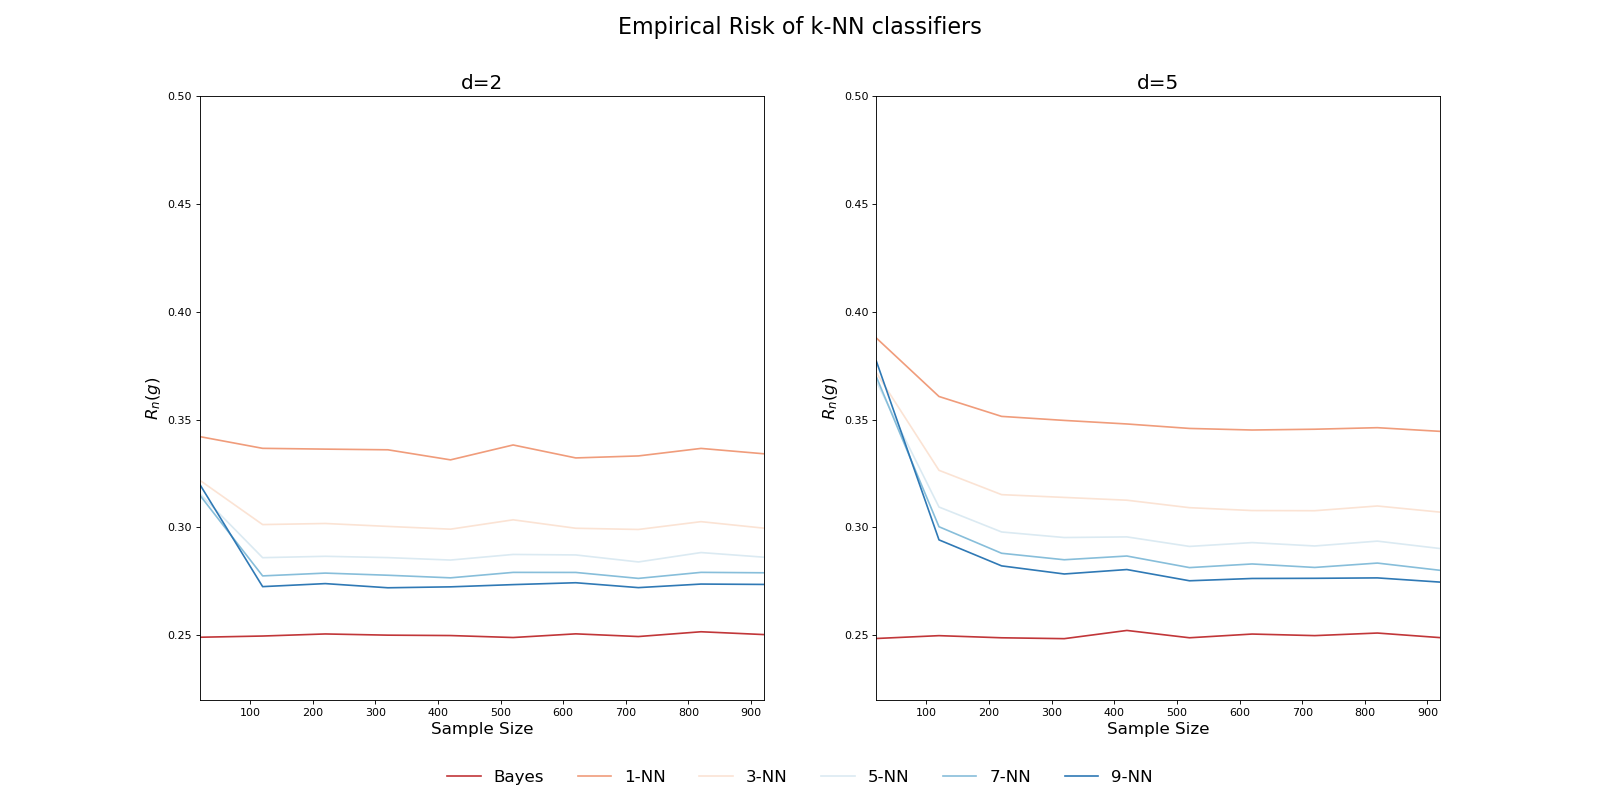
\includegraphics[scale= 0.3]{Emp_Risk_d_2_5}
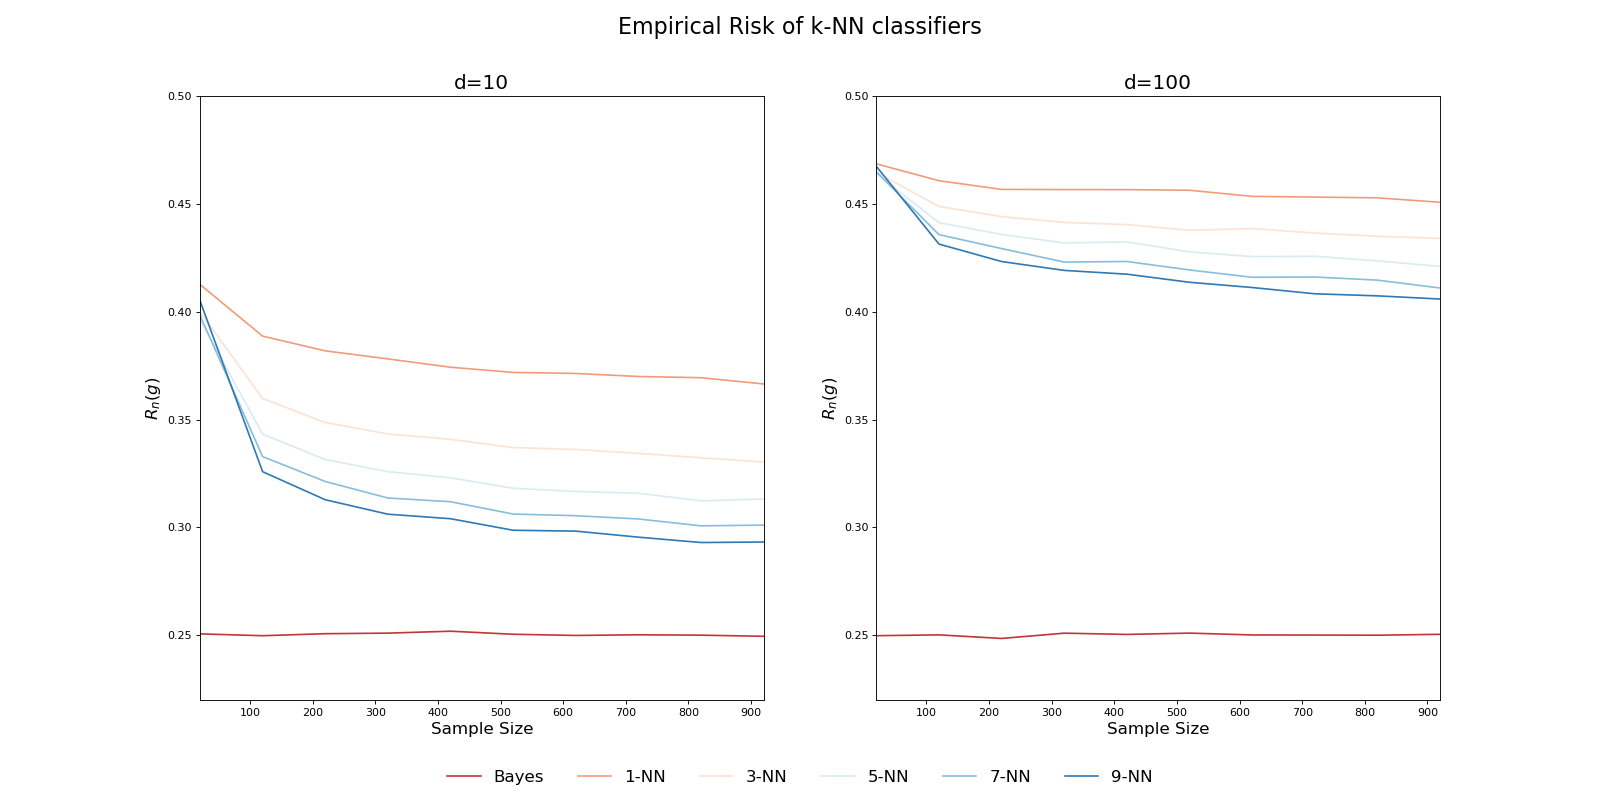
\includegraphics[scale= 0.3]{Emp_Risk_d_10_100}
\end{figure}

For example, in 2 dimensions, the empirical risk of the 3-NN rule converges towards the expected value of 0.3 once the sample size exceeds roughly 100 obvservations. In 5 dimensions, the boundary for convergence is already being pushed to a sample size greater than 500. Similarly, all other k-NN classifiers show higher risk the higher the dimensions. Overall, the risk is lower for greater values of k.

As we've shown in class, if we are in a high dimensional space, the distances between points grow, so for the nearest neighbor to be close and of the same type, we need a massive amount of data. Additionally, we can interpret these outputs as a reminder to not include irrelevant features when building classifiers. The only feature that is relevant for this task is the first entry, all others are just noise. Finally, the Bayes classifier always performs as expected. \\

For the second part, we're essentially testing empirical risk minimization based on cross validation. We use a growing testing set to estimate our risk. We would expect, that with a larger testing set, we'd choose the classifier with the lowest risk more often. This should be the 9-NN Classifier, as shown in the previous simulations. 

\begin{figure}[H]
\centering
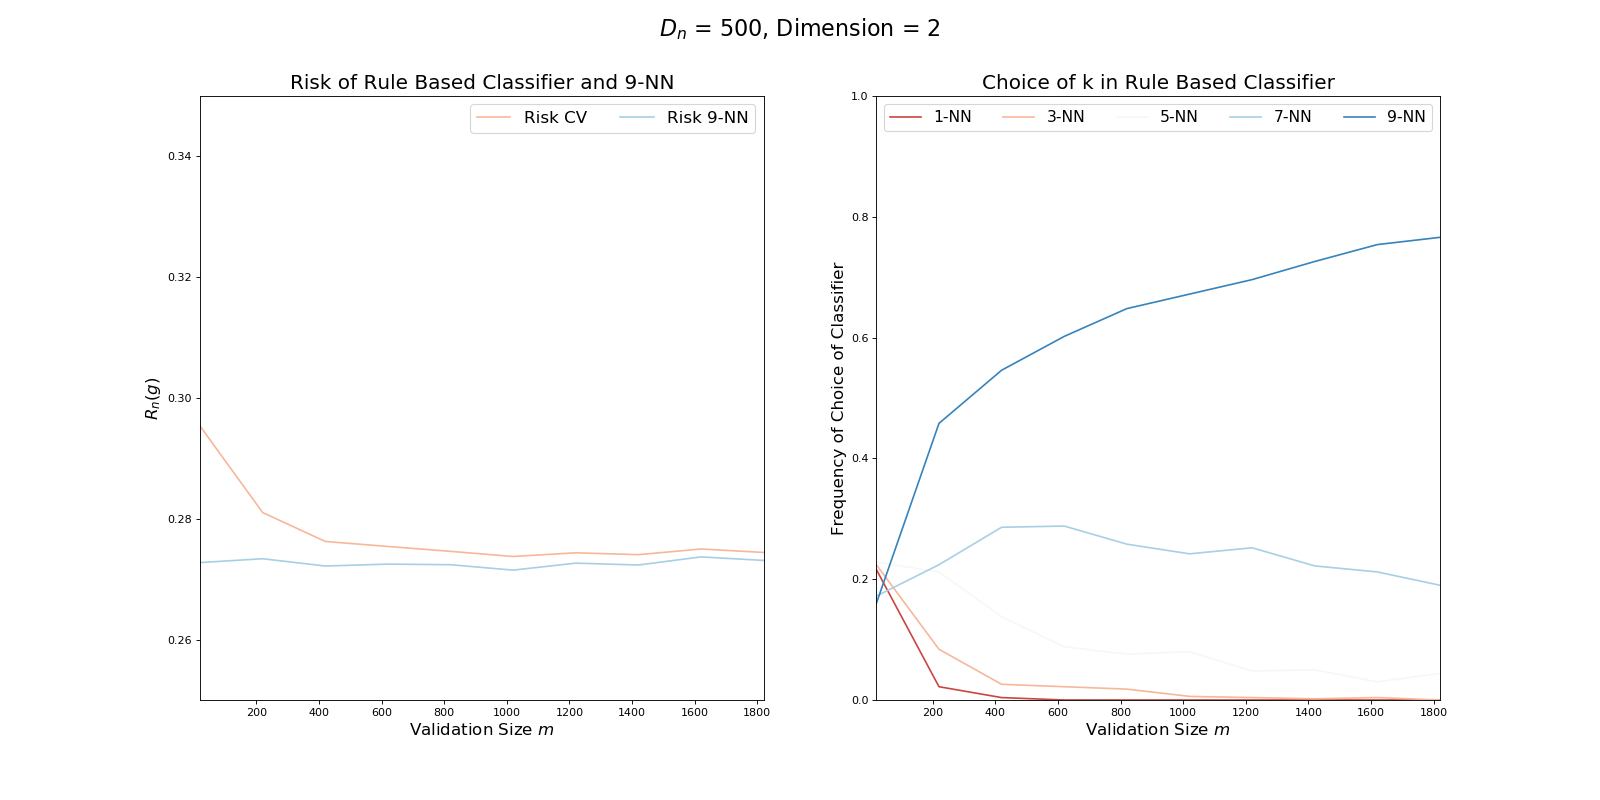
\includegraphics[scale= 0.3]{CV_KNN_n500_d2}
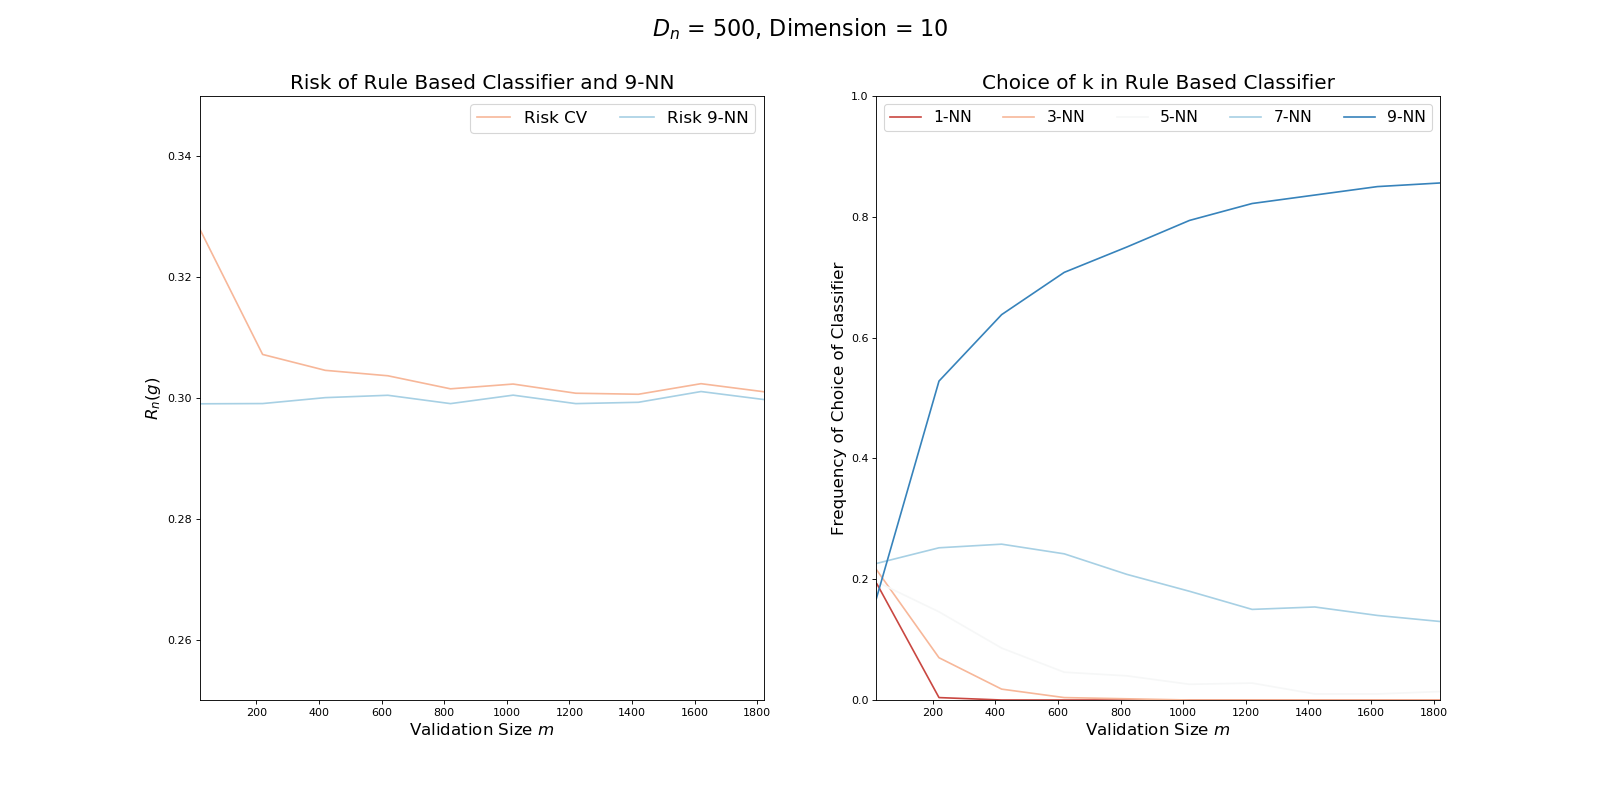
\includegraphics[scale= 0.3]{CV_KNN_n500_d10}
\end{figure}

The plots show repeated simulations for each $m$. Each time the minimum risk classifier is choose based on the testing set $D_m$. The left plot shows the average risk at each $m$ of the classifier choosen by the rule, compared to the average risk of the 9-NN Classifier. Clearly, for lower $m$, the rule doesn't always choose the right classifier. The empirical risk is on average higher than the empirical risk of just choosing the 9-NN Classifier. The left side shows the percentage of times each classifier had the lowest risk in the testing set, at a given $m$ over 500 rounds. Again, as $m$ grows, the 9-NN rule is choosen more often. \\

As discussed in class, we can bound the absolute difference between the empirical risk on a testing set $R _ { m } ^ { \prime } \left( p _ { n } ^ { ( j ) } \right)$ and the true risk of a classifier $R \left( p _ { n } ^ { ( j ) } \right)$ for a class of classifiers $j \in C$. Denoting $N$ the number of classifiers in $C$ we showed that:

$$\left| R _ { m } ^ { \prime } \left( p _ { n } ^ { ( j ) } \right) - R \left( p _ { n } ^ { ( j ) } \right) \right| \leqslant \sqrt { \frac { \log \frac { 2 N } { \delta } } { 2 m } }$$

with probability $\geq 1 - \delta$.\\

So in this case with $N=5$, we could say with 95\% probability, that the absolute difference between the risks is smaller than approx. 0.05 for $m=1000$. Eyeballing the plots, one can see that this seems to hold. 

\end{document}


 